\section{极限存在准则,两个重要极限}
\subsection{夹逼准则}

\begin{example}
证明:\(\lim_{x\to0} \sqrt[n]{1+x} = 1\).
\begin{proof}
当\(x > 0\)时,
因为\(1 < \sqrt[n]{1+x} < 1+x\),
且\(\lim_{x\to0^+} 1 = \lim_{x\to0^+}(1+x) = 1\),
所以\[
	\lim_{x\to0^+} \sqrt[n]{1+x} = 1;
\]

当\(-1 < x < 0\)时,
因为\(1+x < \sqrt[n]{1+x} < 1\),
且\(\lim_{x\to0^-} 1 = \lim_{x\to0^-}(1+x) = 1\),
所以\[
	\lim_{x\to0^-} \sqrt[n]{1+x} = 1.
\]

综上,\(\lim_{x\to0} \sqrt[n]{1+x} = 1\).
\end{proof}
\end{example}

\begin{example}
证明:\(\lim_{x\to0^+} x \floor*{\frac{1}{x}} = 1\).
\begin{proof}
令\(t=1/x\),那么\[
x \floor*{\frac{1}{x}} = \frac{1}{t} \floor{t}.
\]又因为\[
t - 1 < \floor{t} \leq t,
\]\[
1 - \frac{1}{t} < \frac{1}{t} \floor{t} \leq 1;
\]而\[
\lim_{t\to+\infty} 1 - \frac{1}{t} = 1,
\quad
\lim_{t\to+\infty} 1 = 1,
\]所以\[
\lim_{x\to0^+} x \floor*{\frac{1}{x}} = \lim_{t\to+\infty} \frac{1}{t} \floor{t} = 1.
\qedhere
\]
\end{proof}
\end{example}


\subsection{单调有界定理}

相应于单调有界数列必有极限的准则,函数极限也有类似的准则.
\begin{theorem}\label{theorem:极限.函数的单调有界定理}
设函数\(f(x)\)在点\(x_0\)的某个左邻域\((x_0-\delta,x_0)\)内单调并且有界,则\(f(x)\)在\(x_0\)的左极限\(f(x_0^-)\)必定存在.
\end{theorem}

\begin{example}[重要极限II]
试证:极限\(\lim_{x \to \infty}\left(1 + \frac{1}{x}\right)^x\)存在.
\begin{proof}
考虑\(x\)取正整数\(n\)而趋于\(+\infty\)的情形.设\(x_n=\left(1+\frac{1}{n}\right)^n\),根据牛顿二项公式,有\begin{align*}
x_n &= \left(1+\frac{1}{n}\right)^n
= \sum_{k=0}^n \frac{n!}{k! (n-k)!} \frac{1}{n^k} \\
&= 1 + \frac{n}{1!}\frac{1}{n} + \frac{n(n-1)}{2!}\frac{1}{n^2} + \frac{n(n-1)(n-2)}{3!}\frac{1}{n^3} + \dotsb \\
&\qquad+ \frac{n(n-1)\dotsm(n-n+1)}{n!}\frac{1}{n^n} \\
&= 1 + 1 + \frac{1}{2!}\left(1-\frac{1}{n}\right) + \frac{1}{3!}\left(1-\frac{1}{n}\right)\left(1-\frac{2}{n}\right) + \dotsb \\
&\qquad+ \frac{1}{n!}\left(1-\frac{1}{n}\right)\left(1-\frac{2}{n}\right)\dotsm\left(1-\frac{n-1}{n}\right),
\end{align*}
类似地,\begin{align*}
x_{n+1}
&= 1 + 1 + \frac{1}{2!}\left(1-\frac{1}{n+1}\right) + \frac{1}{3!}\left(1-\frac{1}{n+1}\right)\left(1-\frac{2}{n+1}\right) + \dotsb \\
&\qquad+ \frac{1}{n!}\left(1-\frac{1}{n+1}\right)\left(1-\frac{2}{n+1}\right)\dotsm\left(1-\frac{n-1}{n+1}\right) \\
&\qquad+ \frac{1}{(n+1)!}\left(1-\frac{1}{n+1}\right)\left(1-\frac{2}{n+1}\right)\dotsm\left(1-\frac{n}{n+1}\right),
\end{align*}
比较\(x_n\)和\(x_{n+1}\)的展开式,可以看到除前两项外,\(x_n\)的每一项都小于\(x_{n+1}\)的对应项,并且\(x_{n+1}\)还多了最后一项\[
\frac{1}{(n+1)!}\left(1-\frac{1}{n+1}\right)\left(1-\frac{2}{n+1}\right)\dotsm\left(1-\frac{n}{n+1}\right) > 0,
\]因此\[
x_n < x_{n+1},
\]这就说明数列\(\{x_n\}\)是单调增加的.

又因为\[
x_n < 1 + 1 + \frac{1}{2!} + \frac{1}{3!} + \dotsb + \frac{1}{n!}
< 1 + 1 + \frac{1}{2} + \frac{1}{2^2} + \dotsb + \frac{1}{2^{n-1}}
= 3 - \frac{1}{2^{n-1}} < 3,
\]这就说明数列\(\{x_n\}\)是有界的.

既然数列\(\{x_n\}\)是单调增加的,
又是有界的,
那么数列\(\{x_n\}\)的极限一定存在,
记它的极限值为常数\(e\).

再设\(n \leq x < n+1\),则\[
\left(1+\frac{1}{n+1}\right)^n < \left(1+\frac{1}{x}\right)^x < \left(1+\frac{1}{n}\right)^{n+1},
\]且当\(n\to\infty\)时,\(x\to\infty\),而\[
\lim_{n\to\infty}\left(1+\frac{1}{n+1}\right)^n
=\lim_{n\to\infty}\frac{\left(1+\frac{1}{n+1}\right)^{n+1}}{1+\frac{1}{n+1}} = e,
\]\[
\lim_{n\to\infty}\left(1+\frac{1}{n}\right)^{n+1}
=\lim_{n\to\infty}\left[\left(1+\frac{1}{n}\right)^n\cdot\left(1+\frac{1}{n}\right)\right]=e,
\]应用\hyperref[theorem:极限.夹逼准则]{夹逼准则}可得\[
\lim_{x\to+\infty}\left(1+\frac{1}{x}\right)^x = e.
\]令\(x=-(t+1)\),则\(x\to-\infty\)时,\(t\to+\infty\),从而\begin{align*}
\lim_{x\to-\infty}\left(1+\frac{1}{x}\right)^x
&=\lim_{t\to+\infty}\left(1-\frac{1}{t+1}\right)^{-(t+1)}
=\lim_{t\to+\infty}\left(\frac{t}{t+1}\right)^{-(t+1)} \\
&=\lim_{t\to+\infty}\left(1+\frac{1}{t}\right)^{t+1}
=\lim_{t\to+\infty}\left[\left(1+\frac{1}{t}\right)^t\cdot\left(1+\frac{1}{t}\right)\right]=e.
\end{align*}

综上所述,由于\[
\lim_{x\to+\infty}\left(1+\frac{1}{x}\right)^x
= \lim_{x\to-\infty}\left(1+\frac{1}{x}\right)^x
= e,
\]所以\begin{equation}\label{equation:极限.重要极限II}
\lim_{x\to\infty} \left(1+\frac{1}{x}\right)^x = e.
\end{equation}
这就说明函数极限\(\lim_{x\to\infty} \left(1+\frac{1}{x}\right)^x\)存在.
\end{proof}
\end{example}
我们称上面所说的常数\(e\)为“\DefineConcept{欧拉常数} \(e\)”.

另外,利用复合函数的极限运算法则,可得
\begin{equation}
\lim_{z\to0}(1+z)^{\frac{1}{z}}
\xlongequal{z=1/x}
\lim_{x\to\infty}\left(1+\frac{1}{x}\right)^x
= e.
\end{equation}

\begin{figure}[ht]
	\centering
	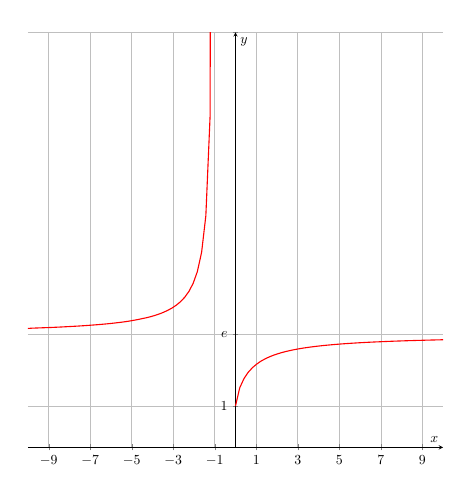
\begin{tikzpicture}[scale=.5]
	% Mathematica: Plot[{E,(1+1/x)^x},{x,-10,10},PlotRange->{0,10},AspectRatio->Automatic,PlotStyle->{{Dashed,Thin},Thin}]
		\begin{axis}[
			xmin=-10,xmax=10,ymin=0,ymax=10,
			grid=both,width=\textwidth,height=\textwidth,
			xlabel=$x$,
			ylabel=$y$,
			enlarge x limits=0.1,
			enlarge y limits=0.1,
			axis lines = middle,
			xtick={-9,-7,...,9},
			ytick={1,2.718,10},
			yticklabels={$1$,$e$},
		]
			\begin{scope}[samples=50,thick,red]
				\addplot[domain=-10:-0]{(1+1/x)^x};
				\addplot[domain=+0:+10]{(1+1/x)^x};
			\end{scope}
		\end{axis}
	\end{tikzpicture}
	\caption{函数\(y=\left(1+\tfrac{1}{x}\right)^x\)的图像}
	\label{figure:极限.函数(1+1/x)^x的图像}
\end{figure}

如\cref{figure:极限.函数(1+1/x)^x的图像} 所示,
我们可以画出函数\(y=\left(1+\frac{1}{x}\right)^x\ (x<-1 \lor x>0)\)的图像.
可见,直线\(y=e\)是函数\(y=\left(1+\frac{1}{x}\right)^x\)的图像的水平渐近线.
另外,易证\[
\lim_{x\to0^+} \left(1+\frac{1}{x}\right)^x = 1,
\qquad
\lim_{x\to1^-} \left(1+\frac{1}{x}\right)^x = +\infty.
\]


\begin{example}
求:\(\lim_{x \to \infty}\left(1 - \frac{1}{x}\right)^x\).
\begin{solution}
令\(t = -x\),则当\(x \to +\infty\)时,\(t \to -\infty\),于是\[
\lim_{x \to +\infty}\left(1 - \frac{1}{x}\right)^x
= \lim_{t \to -\infty}\left(1 + \frac{1}{t}\right)^{-t}
= \lim_{t \to -\infty}\frac{1}{\left(1 + \frac{1}{t}\right)^t}
= \frac{1}{e}.
\]
\end{solution}

画出函数\(y=\left(1-\frac{1}{x}\right)^x\ (x<0 \lor x\geq1)\)的图像如\cref{figure:极限.函数(1-1/x)^x的图像}.
\begin{figure}[ht]
	\centering
	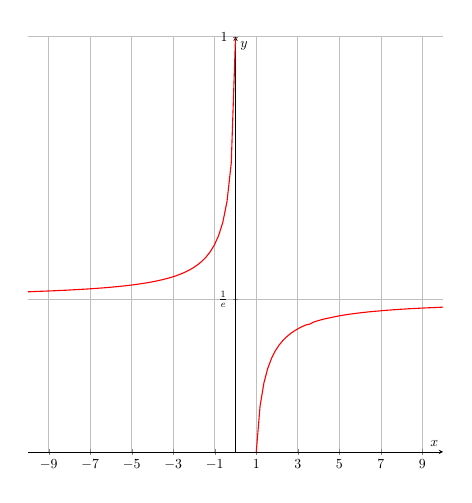
\begin{tikzpicture}[scale=.5]
		% Mathematica: Plot[{1/E, (1 - 1/x)^x}, {x, -10, 10}, PlotRange -> {0, 1}, PlotStyle -> {{Dashed, Thin}, Thin}]
		\begin{axis}[
			xmin=-10,xmax=10,
			ymin=0,ymax=1,
			grid=both,
			width=\textwidth,height=\textwidth,
			xlabel=$x$,
			ylabel=$y$,
			axis lines=middle,
			xtick={-9,-7,...,10},
			ytick={.3679,1},
			yticklabels={$\frac{1}{e}$,$1$},
		]
			\begin{scope}[samples=50,thick,red]
				\addplot[domain=-10:-0]{(1-1/x)^x};
				\addplot[domain=+1:+10]{(1-1/x)^x};
			\end{scope}
		\end{axis}
	\end{tikzpicture}
	\caption{函数\(y=\left(1-\tfrac{1}{x}\right)^x\)的图像}
	\label{figure:极限.函数(1-1/x)^x的图像}
\end{figure}
可见,直线\(y=\frac{1}{e}\)是函数\(y=\left(1-\frac{1}{x}\right)^x\)的图像的水平渐近线.
另外,易证\[
	\lim_{x\to0^-} \left(1-\frac{1}{x}\right)^x
	\xlongequal{t=-1/x} \lim_{t\to+\infty} \frac{1}{\sqrt[t]{1+t}}
	= 1.
\]
\end{example}

类似地,函数极限也有自己的柯西审敛原理.

\begin{definition}\label{definition:极限.函数在集合上的振幅}
%@see: 《数学分析》(卓里奇) P109 定义16.
对于任意一个函数\(f\colon X\to\mathbb{R}\),
集合\(E \subseteq X\),
定义:\[
	\amp(f;E)
	\defeq
	\sup_{x_1,x_2 \in E}\abs{f(x_1)-f(x_2)},
\]
称为“函数\(f\)在集合\(E\)上的\DefineConcept{振幅}”.
\end{definition}

\begin{theorem}\label{theorem:极限.函数的柯西极限存在准则}
函数\(f(x)\)在点\(a\)的极限存在的充分必要条件是:
对于任意给定的正数\(\epsilon\),
存在正数\(\delta\),
使得当\(0 < \abs{x_1 - a} < \delta\)且\(0 < \abs{x_2 - a} < \delta\)时,
就有\(\abs{f(x_1) - f(x_2)} < \epsilon\).
\end{theorem}
